\begin{figure}[htbp]
\section*{ KCNH5}
\centering
\begin{subfigure}[b]{0.95\textwidth}
\centering
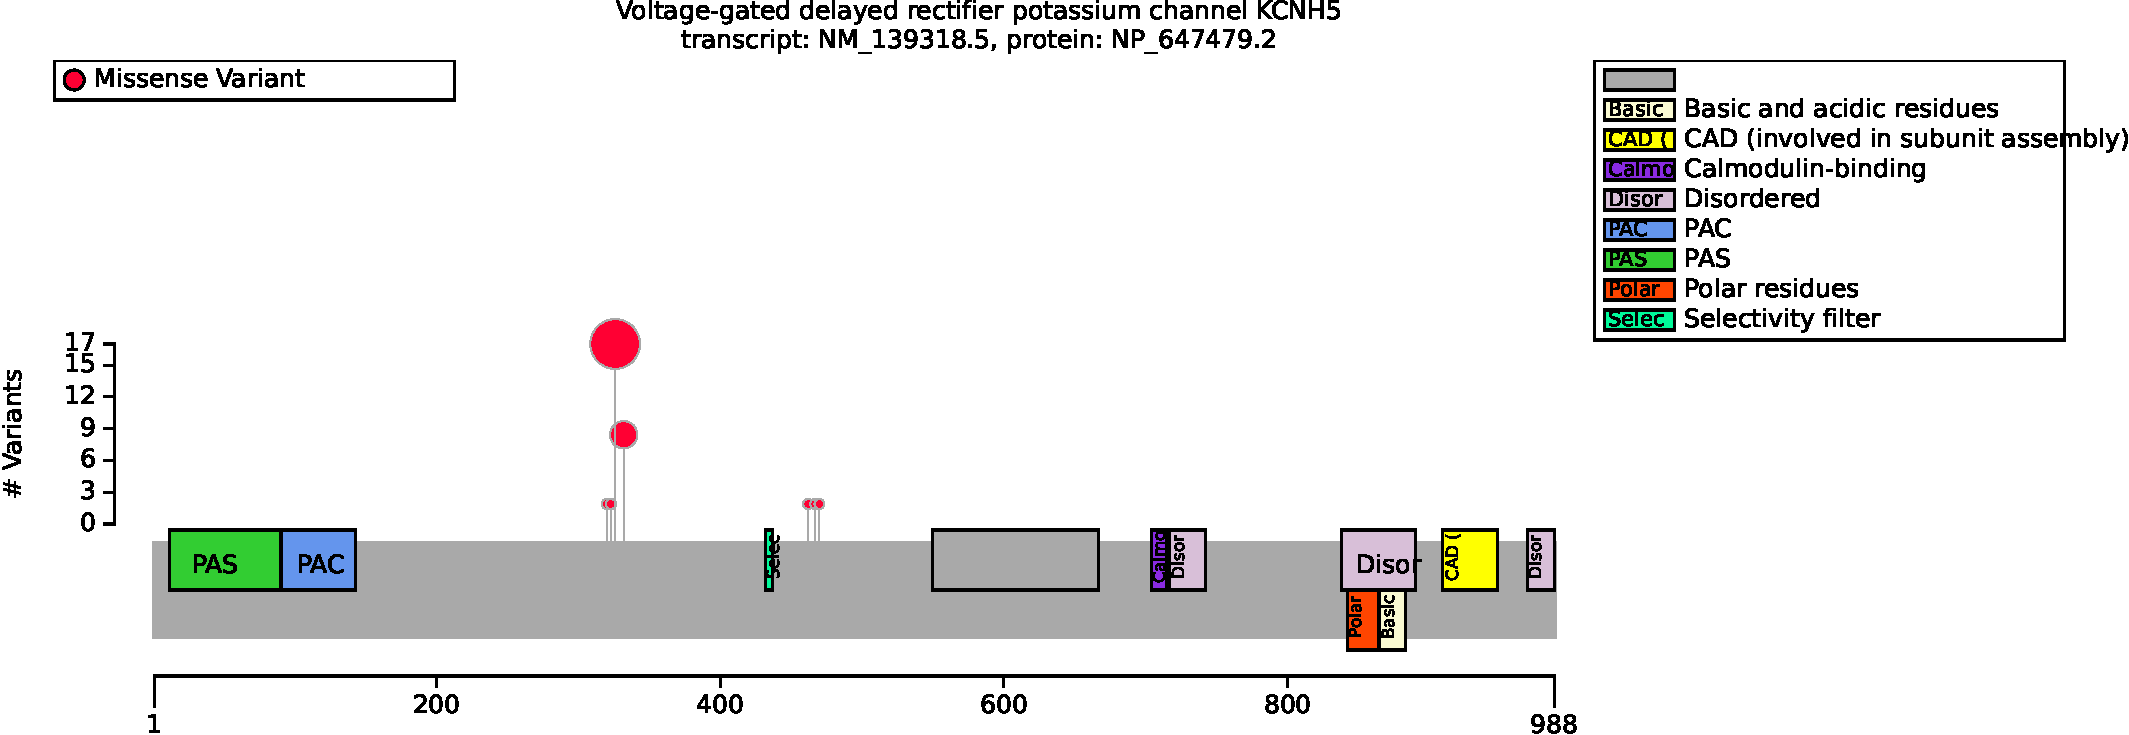
\includegraphics[width=\textwidth]{ img/KCNH5_protein_diagram.pdf} 
\captionsetup{justification=raggedright,singlelinecheck=false}
\caption{Distribution of variants in KCNH5}
\end{subfigure}

\vspace{2em}

\begin{subfigure}[b]{0.95\textwidth}
\centering
\resizebox{\textwidth}{!}{
\begin{tabular}{llllrr}
\toprule
HPO term & Arg327His & Arg333His & p-value & adj. p-value\\
\midrule
Epileptic encephalopathy [HP:0200134] & 15/15 (100\%) & 0/3 (0\%) & 0.001 & 0.016\\
\bottomrule
\end{tabular}
}
\captionsetup{justification=raggedright,singlelinecheck=false}
\caption{Fisher Exact Test performed to compare HPO annotation frequency with respect to Arg327His and Arg333His. Total of
        13 tests were performed.}
\end{subfigure}
\vspace{2em}
\begin{subfigure}[b]{0.95\textwidth}
\centering
\resizebox{\textwidth}{!}{
\begin{tabular}{llllrr}
\toprule
Genotype (A) & Genotype (B) & total tests performed & significant results\\
\midrule
FEMALE & MALE & 17 & 0\\
\bottomrule
\end{tabular}
}
\captionsetup{justification=raggedright,singlelinecheck=false}
\caption{Fisher Exact Test performed to compare HPO annotation frequency with respect to genotypes.}
\end{subfigure}

\vspace{2em}

\caption{ The cohort comprised 27 individuals (14 females, 13 males). A total of 28 HPO terms were used to annotate the cohort. Disease diagnosis: Developmental and epileptic encephalopathy 112 (OMIM:620537). Two recurrent variants have been reported, p.Arg327His and p.Arg333His, both of which are located in or near the functionally critical 
voltage-sensing or pore domains. Happ et al (2023) state that in their cohort, Individuals with the recurrent p.Arg333His variant had a self-limited 
drug-responsive focal or generalized epilepsy and normal intellect, whereas the recurrent p.Arg327His variant was associated with infantile-onset DEE \cite{PMID_36307226}. 
A total of 27 unique variant alleles were found in \textit{KCNH5} (transcript: \texttt{NM\_139318.5}, protein id: \texttt{NP\_647479.2}).}
\end{figure}
